Given the data matrix
\[
    \textbf{X}
    =
    \begin{bNiceArray}{rr}
        3 & 4 \\
        6 & -2 \\
        3 & 1
    \end{bNiceArray}
\]
\begin{enumerate}[label=(\alph*)]
    \item Graph the scatter plot in $p=2$ dimensions. Locate the sample mean on the diagram.
    \begin{lstlisting}
        X = [3 4; 6 -2; 3 1];
        mean_pt = mean(X);
        hold on
            % Plot data.
            scatter(X(:,1),X(:,2),'blue','filled')
            % Plot mean.
            plot(mean_pt(1),mean_pt(2),'d')
            % Text for mean.
            text(mean_pt(1)+0.5,mean_pt(2)+0.2, ...
                join(["$$\bar{x}=\left[\begin{array}{c}",mean_pt(1),"\\",mean_pt(2),"\end{array}\right]$$"],''), ...
                'interpreter','latex')
            % Text for data.
            for r = 1:height(X)
                anno = join(["$$x_",r," = \left[\begin{array}{c}",X(r,1),"\\",X(r,2),"\end{array}\right]$$"],'');
                text(X(r,1)-1.5,X(r,2)-0.5,anno,'interpreter','latex');
            end
            xlim([0 10])
            ylim([-5 5])
            saveas(gcf,'sol3.2a.png')
        hold off
    \end{lstlisting}

    \begin{figure}[H]
        \centering
        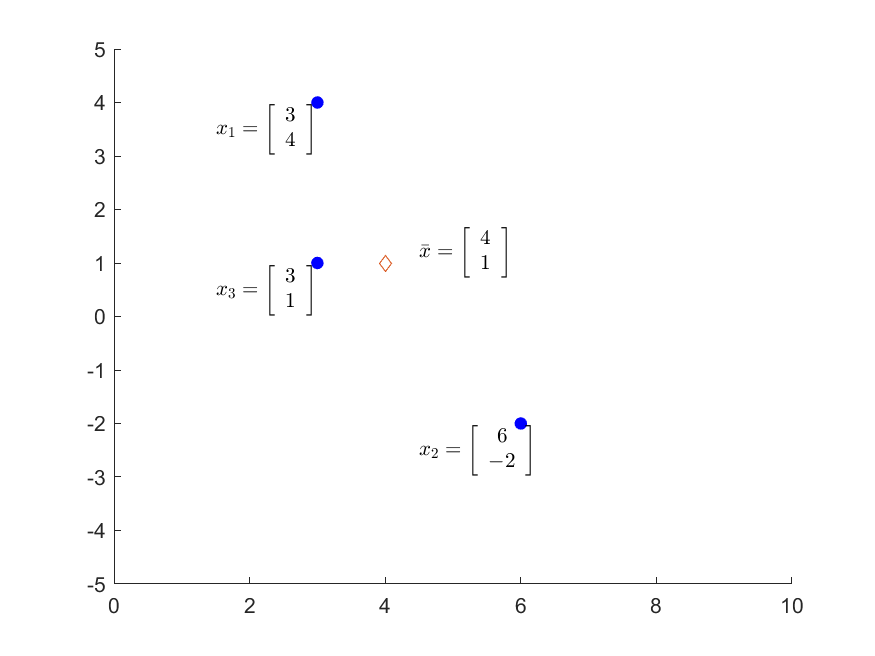
\includegraphics[scale=0.5]{./matlab/chapter-3/sol3.2a.png}
    \end{figure}
    \item Sketch the $n=3$-dimensional representation of the data, and plot the deviation vectors $\textbf{y}_1 - \bar{x}_1\textbf{1}$ and $\textbf{y}_2 - \bar{x}_2\textbf{1}$.
    \[
        \textbf{y}_1 - \bar{x}_1\textbf{1}
        =
        \begin{bNiceArray}{c}
            3 \\
            6 \\
            3
        \end{bNiceArray}
        -
        \begin{bNiceArray}{c}
            4 \\
            4 \\
            4
        \end{bNiceArray}
        =
        \begin{bNiceArray}{r}
            -1 \\
            2 \\
            -1
        \end{bNiceArray}
    \]
    \[
        \textbf{y}_2 - \bar{x}_2\textbf{1}
        =
        \begin{bNiceArray}{c}
            4 \\
            -2 \\
            1
        \end{bNiceArray}
        -
        \begin{bNiceArray}{c}
            1 \\
            1 \\
            1
        \end{bNiceArray}
        =
        \begin{bNiceArray}{r}
            3 \\
            -3 \\
            0
        \end{bNiceArray}
    \]
    \begin{lstlisting}
        % Continuing from part (a)...
        % Compute the deviation vectors.
        d1 = X(:,1) - mean_pt(1)*ones([3,1]);
        d2 = X(:,2) - mean_pt(2)*ones([3,1]);
        % Combine the data with the deviation vectors. First two rows are data,
        % second two are the deviation vectors.
        D = [X d1 d2]';
        start = zeros(size(D));
        
        % Plot the y_1 and y_2 vectors and the d_1, d_2 deviation vectors.
        quiver3(start(:,1), start(:,2), start(:,3), D(:,1), D(:,2), D(:,3));
        % Text for data.
        for r = 1:height(D)
            if r < 3
                % Labels for the data, y_1 and y_2.
                anno = join(["$$\textbf{y}_",r," = \left[\begin{array}{c}",D(r,1),"\\",D(r,2),"\\",D(r,3),"\end{array}\right]$$"],'');
                text(D(r,1)-0.5,D(r,2)-0.2,D(r,3)-0.2,anno,'interpreter','latex');
            else
                % Labels for the deviation vectors, d_1 and d_2.
                anno = join(["$$\textbf{d}_",r-2," = \left[\begin{array}{c}",D(r,1),"\\",D(r,2),"\\",D(r,3),"\end{array}\right]$$"],'');
                text(D(r,1)-0.5,D(r,2)-0.2,D(r,3)-0.2,anno,'interpreter','latex');
            end
        end
    \end{lstlisting}

    \begin{figure}[H]
        \centering
        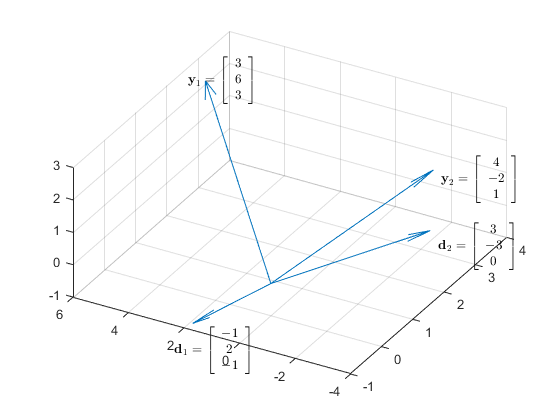
\includegraphics[scale=0.5]{./matlab/chapter-3/sol3.2b.png}
    \end{figure}
    \item Sketch the deviation vectors in (b) emanating from the origin. 
    Calculate the lengths of these vectors and the cosine of the angle between them. 
    Relate the quantities to $\textbf{S}_n$ and $\textbf{R}$.
    \newline
    \par
    The sketch of $\textbf{d}_1$ and $\textbf{d}_2$ are in part (b). The lengths are
    \[
        \left\|\textbf{d}_1\right\|
        =
        \sqrt{{(-1)}^2 + {(2)}^2 + {(-1)}^2}
        =
        \sqrt{1+4+1}
        =
        \sqrt{6}
    \]
    \[
        \left\|\textbf{d}_2\right\|
        =
        \sqrt{{(3)}^2 + {(-3)}^2 + {(0)}^2}
        =
        \sqrt{18}
    \]
    \[
        \mathbf{d}_1 \cdot \mathbf{d}_2
        =
        \begin{bNiceArray}{rrr}
            -1 & 2 & -1
        \end{bNiceArray}
        \begin{bNiceArray}{r}
            3 \\
            -3 \\
            0
        \end{bNiceArray}
        =
        -9
    \]
    \[
        \cos\theta
        =
        \frac{\mathbf{d}_1 \cdot \mathbf{d}_2}{\left\|\textbf{d}_1\right\| \left\|\textbf{d}_2\right\|}
        =
        \frac{-9}{\sqrt{6}\sqrt{18}}
    \]
    \[
        \Rightarrow
        \theta
        =
        {\cos}^{-1}\left(\frac{-9}{\sqrt{32}\sqrt{2}}\right)
        =
        {\cos}^{-1}\left(\frac{-9}{\sqrt{108}}\right)
        =
        {\cos}^{-1}\left(\frac{-3}{\sqrt{12}}\right)
        =
        {\cos}^{-1}\left(\frac{-\sqrt{3}}{2}\right)
        =
        150\degree
    \]
    \par
    For $\textbf{S}_n$, element $s_{12} = \frac{1}{n}{\left(\textbf{y}_1 - \bar{x}_1\textbf{1}\right)}^\prime{\left(\textbf{y}_2 - \bar{x}_2\textbf{1}\right)} = \frac{1}{n}\textbf{d}_1\cdot\textbf{d}_2$, so what we computed for $\textbf{d}_1\textbf{d}_2$ = $n\times s_{12}$. For $\textbf{R}$, when using $\textbf{S}_n$, element $r_{12} = \frac{s_{12}}{\sqrt{s_{22}}\sqrt{s_{22}}} = \frac{(\textbf{d}_1\cdot\textbf{d}_2/n)}{\sqrt{\textbf{d}_1\cdot\textbf{d}_1/n}\sqrt{\textbf{d}_2\cdot\textbf{d}_2/n}} = \frac{(\textbf{d}_1\cdot\textbf{d}_2)}{\sqrt{\textbf{d}_1\cdot\textbf{d}_1}\sqrt{\textbf{d}_2\cdot\textbf{d}_2}}$
\end{enumerate}